
\chapter{Lunedì 29/03/2021 e Martedì 30/03/2021}
\section{Concludiamo su compilatore, assemblatore e collegatore} 
Oggi concludiamo la parte sul compilatore esaminando in modo più organico alcune questioni.
\begin{itemize}
	\item Per creare un programma si può partire da vari sorgenti, che possono essere scritti in c++, ma anche in Assembler. Si aggiungono librerie \emph{statiche} (vedremo a breve) con formato \emph{a}. 
	\item Tutti questi files, da noi introdotti, sono files di testo che passano da vari strumenti. Per quanto riguarda il C++
	\begin{itemize}
		\item preprocessore (ottengo un file cpp in cui le direttive sono state processate)
		\item compilatore (il risultato è un file Assembler)
		\item assemblatore (il risultato è un file oggetto)
	\end{itemize}
	\item I files oggetto e le librerie vanno in ingresso nel collegatore, che produce l'eseguibile.
	\item In linux si utilizza un unico formato per librerie, files oggetto ed eseguibili.
\end{itemize}\begin{center}
	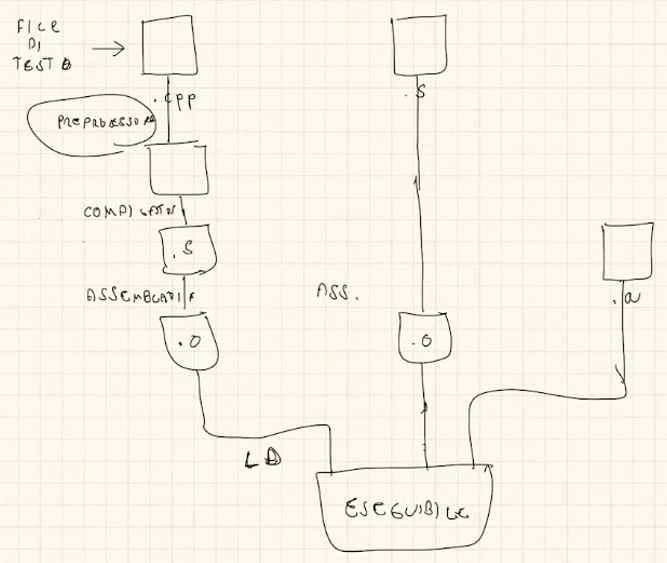
\includegraphics[scale=0.62]{img/50.PNG}
\end{center}  
\subsection{Preprocessore}
Prendiamo un programma C++ (la funzione \emph{foo} è definita in un altro file assembler, che non ci interessa)
\begin{verbatim}
	#include "lib.h"
	
	long var1 = 0;
	long var2 = 4;
	
	int main() {
		// UN COMMENTO
		var1 = foo(var2);
		return var1;
	}
\end{verbatim}
Tutti i file in UNIX sono semplicemente sequenze di byte, l'interpretazione di un file dipende dallo strumento utilizzato per esaminarlo. Col seguente strumento
\begin{verbatim}
	hexdump -vC main.cpp
\end{verbatim}
esaminiamo il file leggendone i corrispondenti esadecimali (la cosa più vicina all'analisi del file nel suo formato binario).\begin{center}
	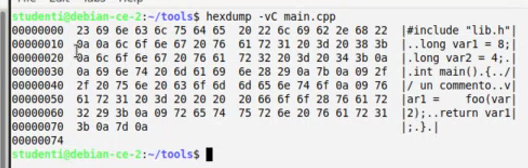
\includegraphics{img/51.PNG}
\end{center}  
\begin{itemize}
	\item La prima colonna da sinistra rappresenta l'offset rispetto al file
	\item Con l'opzione -vC chiedo la stampa a fianco del contenuto del file (se i caratteri sono stampabili, solitamente pone un punto se il carattere non è stampabile\footnote{Tra i caratteri non stampabili c'è quello per andare a capo.}).
\end{itemize}
\subsubsection{Analisi di quanto fatto dal preprocessore} Possiamo chiedere a g++ di fermarsi subito dopo il preprocessore
\begin{verbatim}
	g++ -E main.cpp
\end{verbatim}
L'output risultante, dal programma precedente è il seguente...
\begin{verbatim}
	# 1 "main.cpp"
	# 1 "<built-in>"
	# 1 "<command-line>"
	# 1 "/usr/include/stdc-predef.h" 1 3 4
	# 1 "<command-line>" 2
	# 1 "main.cpp"
	# 1 "lib.h" 1
	long foo(long);
	void bar();
	# 2 "main.cpp" 2
	
	long var1 = 0;
	long var2 = 4;
	
	int main() {
		var1 = foo(var2);
		return var1;
	}
\end{verbatim}
\begingroup
\begin{itemize}
	\item Le prime righe sono informazioni su quanto fatto dal preprocessore, il compilatore le ignorerà.
	\item Osserviamo che la riga di inclusione di \emph{lib.h} è stata sostituita col contenuto del file stesso. 
	\item Sono stati rimossi i commenti, che servono solo a noi.
	\item Ha eliminato lunghe sequenze di spazi bianchi
	\item Le seguenti righe
	\begin{verbatim}
		# 1 "lib.cpp" 1
		...
		# 2 "main.cpp" 2
		...
	\end{verbatim}
	indicano che si sono inclusi questi due files. i numeri in fondo indicano che il preprocessore ha incontrato il file per la prima e la seconda volta, rispettivamente. Col primo numero, invece, indichiamo da quale riga stiamo ripartendo con le successive righe di codice.
\end{itemize}
Il formato è più canonico: sono state rimosse cose che non servono al compilatore, inoltre si è obbedito alle direttive indicate. Un tempo il preprocessore era effettivamente indipendente dal compilatore: questa cosa va bene per il C, ma risulta una cosa molto costosa nel C++. Poichè il preprocessore deve fare un parsing per considerare il file, come il compilatore, si è preferito integrare il preprocessore nel compilatore: un solo parsing per tutto.
\endgroup
\subsubsection{Inclusione di files} Attenzione all'inclusione di files: certe volte viene fatta con virgolette, altre volte con parentesi angolari.
\begin{verbatim}
	#include "lib.h"
	#include <lib.h>
\end{verbatim}
\begin{itemize}
	\item Nel primo caso si indica di cercare il file nella stessa directory del file che stiamo preprocessando, e solo dopo guardare una serie di directories predefinite.
	\item Nel secondo caso si indica di cercare il file solo nelle directory predefinite (vengono usate per evitare il problema di nomi di file uguali a quelli di librerie presenti nelle directories predefinite).
\end{itemize}
\subsubsection{Definizione di macro}
Se noi scriviamo una macro denominata \emph{PIPPO}
\begin{verbatim}
	#include "lib.h"
	#define PIPPO var1
	...
	int main() {
		... var1 = foo(PIPPO); ...
	}
\end{verbatim}
il preprocessore interviene restituendo quanto segue
\begin{verbatim}
	long foo(long);
	void bar();
	...
	int main() {
		... var1 = foo(var1); ...
	}
\end{verbatim}
Si pone \emph{var1} ovunque sia presente \emph{PIPPO} (in questo caso si sostituisce ponendo var1 come nome di una variabile, e non come una stringa).

\subsubsection{Inclusione condizionale di parti di testo} Possiamo includere o meno parti di codice secondo due criteri:
\begin{enumerate}
	\item l'aver definito o no una macro
	\begin{verbatim}
		#include "lib.h"
		#ifdef DEBUG
		void debug(const char*);
		#else
		#define debug(msg);
		#endif
		...
		int main() {
			... 
			var1 = foo(PIPPO);
			debug("questo e' un messaggio di debug");
			...
		}
	\end{verbatim}
	\begin{itemize}
		\item \textbf{Cosa succede se non ho definito la macro DEBUG?}
		\begin{itemize}
			\item La funzione \emph{debug} non esiste.
			\item La direttiva 
			\begin{verbatim}
				#define debug(msg)
			\end{verbatim}
			sostituisce la chiamata di funzione \emph{debug} con il niente (ricordarsi la sintassi della direttiva con cui si definisce una macro).
		\end{itemize}
		\item \textbf{Cosa succede se definisco la macro DEBUG?}
		\begin{itemize}
			\item Poniamo in cima
			\begin{verbatim}
				#define DEBUG 1
			\end{verbatim}
			\item Viene inclusa la riga con cui viene dichiarata la funzione.
			\item La macro con cui si eliminano le chiamate di funzione non viene applicata.
		\end{itemize}
	\end{itemize}
	
	\item avere una macro con un certo valore o no
	\begin{verbatim}
		#if DEBUG == 1
		...
		#endif
	\end{verbatim}
\end{enumerate}
\subsubsection{Macro predefinite}
Col seguente comando possiamo caricare una lista di macro predefinite
\begin{verbatim}
	g++ -E -dM main.cpp
\end{verbatim}
sono tante e definite in base a tanti fattori.
\paragraph{Esempi di macro}
\begin{itemize}
	\item \emph{$\_$linux$\_$}, se mi trovo su linux o meno;
	\item \emph{$\_$x86$\_$64$\_$}, se viene utilizzata l'omonima architettura...
\end{itemize}
\subsubsection{Curiosità: eredità dell'indipendenza del preprocessore}
Un esempio di eredità dell'indipendenza del preprocessore dal compilatore l'abbiamo con la seguente riga
\begin{verbatim}
	#define DEBUG 1;
\end{verbatim}
il punto e virgola, che è parte della sintassi del C++, viene considerato parte del valore della macro \emph{DEBUG}.
\clearpage
\subsection{Assemblatore}
L'assemblatore, essenzialmente, prepara il contenuto di sezioni di memoria:
\begin{itemize}
	\item \emph{data} e \emph{text}, che già conosciamo;
	\item \emph{bss}, sezione dove saranno collocate le variabili globali che hanno come valore zero. Nel file viene indicata la sola dimensione, non il contenuto (ovviamente).
\end{itemize} 
\paragraph{Come lavora l'assemblatore?} L'assemblatore lavora concettualmente con due passate: diciamo concettualmente perché non è detto che la cosa avvenga, fisicamente parlando. Parlare in questo modo è un'eredità del passato, quando il calcolatore doveva leggere per forza il programma due volte (pensare alle schede perforate, si dovevano fare due letture per estrarre delle informazioni, cosa necessaria visto che la memoria all'epoca era poca).
\begin{itemize}
	\item Nella prima "passata concettuale" crea una tabella dei simboli, ogni volta che trova una nuova etichetta aggiunge una nuova entrata. Per ogni sezione mantiene un contatore, per ricordarsi il numero di byte effettivamente utilizzati in quella sezione. Per ogni etichetta individuata memorizza a quanto era arrivato il contatore: l'offset del corrispondente byte all'interno della sezione in cui l'etichetta è stata definita.
	\item Nella seconda passata traduce effettivamente il programma, crea i byte da porre nelle varie sezioni, utilizzando la tabella dei simboli. 
\end{itemize}
Questa divisione concettuale in due passate permette di utilizzare etichette definite successivamente: contrariamente al C++ non dobbiamo dichiarare un'etichetta prima di usarla, è un qualcosa che è necessario per dare senso alle istruzioni JMP.

\subsection{Formato ELF (\emph{Executable and Linking Format})} Abbiamo un file binario\footnote{Se facciamo l'\emph{hexdump} del formato oggetto individuiamo sequenze esadecimali molto lunghe, e poche cose stampabili.} in formato ELF (\emph{Executable and Linking Format}). Il formato è comune per files oggetto, librerie statiche ed eseguibili.
\paragraph{Struttura stabilita dal formato ELF}\begin{center}
	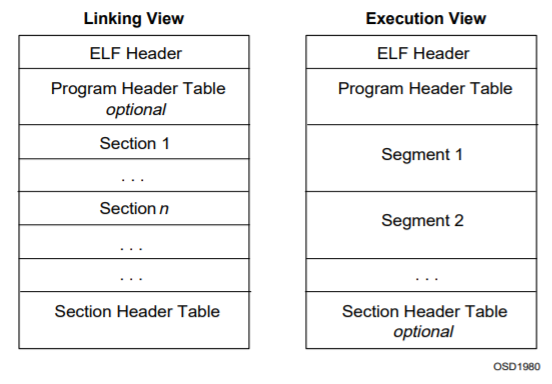
\includegraphics[scale=0.8]{img/52.PNG}
\end{center}  
\begin{itemize}
	\item Intestazione ELF, unica parte fissa 
	\item Parte rimanente, variabile e interpretabile in base al contenuto dell'intestazione. Il file ELF permette una doppia visione in base all'uso che si deve fare (ricordiamo che funge come file oggetto o eseguibile).
	\begin{itemize}
		\item Gli strumenti interessati alla rilocazione (collegatore) prendono una \textbf{\emph{tabella delle sezioni}}, che permette di recuperare le sezioni all'interno del file.
		\item Gli strumenti interessati all'esecuzione del file prendono una \textbf{\emph{tabella del programma}} (o \emph{tabella dei segmenti}), che indica i segmenti presenti nel file, come devono essere caricati e utilizzati.
		\item Attenzione all'\emph{optional}: per i primi è facoltativa la cosa richiesta dai secondi, e viceversa.
	\end{itemize}
\end{itemize}
\paragraph{Esaminare un file ELF} Esistono degli strumenti che permettono di esaminare i file ELF in maniera più comoda. Uno di questi lo abbiamo già utilizzato: l'\emph{objdump}.
\begin{verbatim}
	objdump -o foo.o
\end{verbatim}
Il programma non è specifico per i files ELF, quindi alcune cose non è in grado di interpretarle, o le interpreta in modo strano. Uno strumento più adatto è \emph{readelf}. Scrivendo il seguente comando
\begin{verbatim}
	readelf -h foo.o
\end{verbatim}
siamo in grado di leggere, in modo chiaro, le informazioni codificate nell'intestazione ELF.\begin{center}
	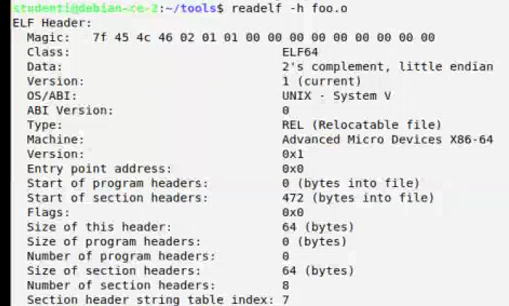
\includegraphics{img/53.PNG}
\end{center}  
\begin{itemize}
	\item Attenzione a quel \emph{magic number}: è l'inizio di ogni file ELF, un identificativo dei files ELF. 
	\item Tra le cose presenti abbiamo:
	\begin{itemize}
		\item Informazioni sul sistema per cui è realizzato il programma.
		\item Punto di partenza della tabella delle sezioni e della tabella dei programmi: il fatto che si abbia una tabella all'offset 0 ne stabilisce la sua assenza (all'offset zero è presente, per forza, il \emph{magic number} detto prima).
		\item Numero di sezioni presenti e dimensione di ciascuna sezione (sostanzialmente è come un'array). Il formato, con lo scopo di essere il più generico possibile, non fissa numero di elementi presenti e dimensione degli stessi. In questo caso abbiamo 8 entrate, ciascuna da 64bit.
	\end{itemize}
\end{itemize}
\subsubsection{Tabella delle sezioni} Possiamo chiedere a \emph{readelf} di mostrarci la tabella delle sezioni, col seguente comando
\begin{verbatim}
	readelf -WS foo.o
\end{verbatim}
\begin{center}
	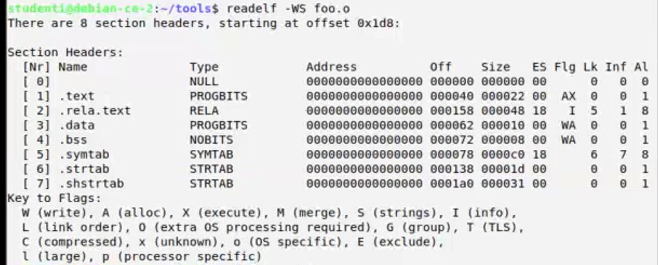
\includegraphics[scale=.9]{img/54.PNG}
\end{center}  
La sezione 0 è sempre nulla. Quali informazioni abbiamo per ciascuna sezione?
\begin{itemize}
	\item Il nome, che è una stringa (le entrate con lunghezza fiscca non danno problemi, contrariamente a quelle con lunghezza variabile). Per le stringhe si è deciso di riservare un'area dove queste vengono poste in sequenza (\emph{strtab}, \emph{shstrtab}), una dopo l'altra. Le entrate in dimensione fissa sono identificate immediatamente da un offset.
	\item Il tipo della sezione è un codice numerico, decodificato da readelf con una stringa. \emph{PROGBITS} sono aree definite dal programmatore, altri tipi come \emph{SYMTAB} e \emph{STRTAB} sono definiti dallo standard.
	\item L'indirizzo dove la sezione viene caricata (l'assemblatore non lo sa, quindi tutto uguale a zero per ora).
	\item L'offset all'interno del file, dove si trova la sezione.
	\item Altre informazioni non significative per tutte le sezioni. Una di queste è il \emph{flag}, che in un certo senso dice cosa si dovrà fare con quella sezione. \textbf{Sotto la tabella delle sezioni è presente una legenda} che suggerisce il significato dei vari flag. Vediamo alcuni esempi
	\begin{itemize}
		\item \textbf{AX}: dobbiamo allocare spazio (A), e quanto allocato dovrà essere eseguibile (X).
		\item \textbf{WA}: dobbiamo allocare spazio (A), e quanto allocato dovrà essere scrivibile (W).
	\end{itemize}
\end{itemize}
\subsubsection{Sezione \emph{symtab}: Tabella dei simboli} Possiamo chiedere a \emph{readelf} di mostrarci la tabella delle sezioni (\emph{syntab})
\begin{verbatim}
	readelf -s foo.o
\end{verbatim}
\begin{center}
	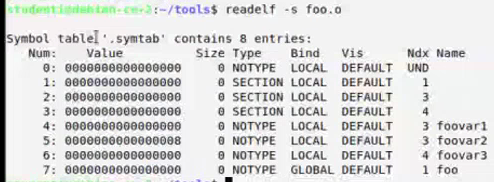
\includegraphics{img/55.PNG}
\end{center}  
Quali informazioni abbiamo in ciascuna entrata?
\begin{itemize}
	\item Il nome del simbolo (nelle sequenze di bit relative alla tabella non si pone di nuovo il nome, ma l'offset relativo a \emph{syntab} dove possiamo trovare il nome).
	\item Il valore, che consiste (in questo momento della compilazione) nell'offset del simbolo all'interno della sezione in cui è definito.
	\item \emph{Ndx}, identificativo della sezione in cui si trova il simbolo.
	\item Dimensione e tipo del simbolo, non rilevanti per quanto ci riguarda.
	\item \emph{Bind}, se il dato ha visibilità locale o globale.
\end{itemize}
\subsubsection{Sezione \emph{rela.section$\_$name}: tabella di rilocazione} Abbiamo già visto col seguente comando
\begin{verbatim}
	objdump -d foo.o
\end{verbatim}
che l'assemblatore non conosce il valore del simboli. Si riservano aree mettendo come valori zero, e si lascia la palla al linker. Queste cose sono gestite mediante \emph{tabelle di rilocazione}: ne produce una per ogni sezione che ne ha bisogno. La sezione è di tipo \emph{RELA} (\emph{Rilocazione con addendo}), attenzione al flag \emph{I}, la tabella contiene informazioni per il linker). Nel nostro esempio la tabella è stata creata solo per la sezione \emph{text}: si dice al linker come modificare la sezione \emph{text} quando il valore di tutti i simboli sarà conosciuto. Leggiamo il contenuto col seguente comando
\begin{verbatim}
	readelf -r foo.o
\end{verbatim}
\begin{center}
	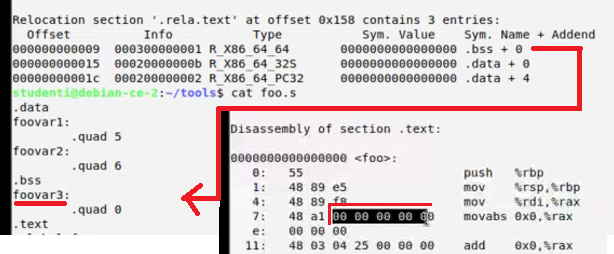
\includegraphics{img/57.PNG}
\end{center}  
\begin{itemize}
	\item All'offset 9 della sezione \emph{text} c'è da fare l'operazione \emph{64} (la parte iniziale del tipo è un prefisso legato al processore che stiamo utilizzando), cioè mettere un numero da 64bit a partire da questo offset. Quale numero? Un'operazione, in genere, fa riferimento un simbolo. Nel caso delle rilocazioni con addendo si procede sommando una costante a un simbolo. In questo caso abbiamo $\text{.bss } + 0$ (cioè \emph{foovar3}): si chiede al linker di scrivere a partire dall'offset 9 della sezione \emph{text} quando conoscerà il valore presente in $\text{.bss } + 0$.
\end{itemize}
\subsection{Collegatore}
Cosa fa il collegatore? Scriviamo il seguente comando
\begin{verbatim}
	ld -o main main2.o foo.o
\end{verbatim}
Abbiamo due file oggetto, ciascuno con una sezione \emph{text}, \emph{data}, \emph{bss}. La prima cosa che deve fare il linker è creare un qualcosa di unico: otterremo un'unica sezione \emph{text}, un'unica sezione \emph{data}, un'unica sezione \emph{bss} (che saranno le sezioni del programma finale). La cosa viene fatta prendendo le varie sezioni nell'ordine in cui le abbiamo poste, in base al tipo.\begin{center}
	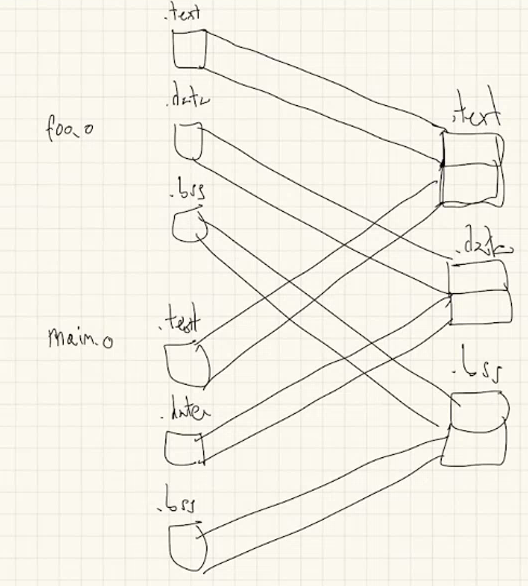
\includegraphics[scale=.85]{img/58.PNG}
\end{center}  
\begin{itemize}
	\item A questo punto il collegatore conosce la dimensione di ogni cosa, dunque può decidere gli indirizzi di partenza di ogni sezione. Pone le sezioni nell'ordine visibile nell'immagine, e ne decide gli indirizzi. 
	\item Se io conosco l'indirizzo di partenza di ogni sezione sarò in grado di raggiungere ogni simbolo.  Il linker, tenendo conto dei vari \emph{symtab} (uno per file), deve intervenire aggiustando i vari \emph{offset} relativi alle sezioni successive alla prima. Ottengo una tabella dei simboli finale.
	\item Tra questi simboli potrebbero esserci simboli non definiti. Il file finale, affinchè sia eseguibile, non deve avere simboli non definiti (ciò che non è stato definito in un file deve essere per forza definito da qualche altra parte).
	\item A questo punto possono essere eseguite tutte le istruzioni di rilocazione seguendo le informazioni presenti nella \emph{tabella di rilocazione}.
\end{itemize}
\paragraph{Informazioni nell'intestazione ELF dopo aver collegato tutto} Scriviamo 
\begin{verbatim}
	readelf -h main
\end{verbatim}
\begin{center}
	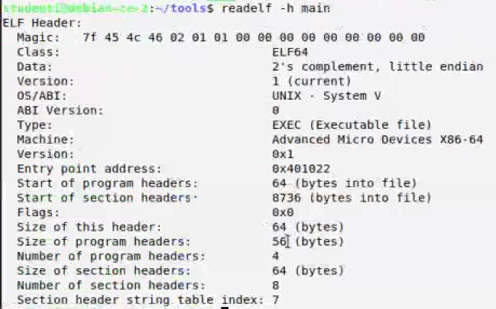
\includegraphics{img/59.PNG}
\end{center}  
\begin{itemize}
	\item Il tipo è cambiato: abbiamo un eseguibile (\emph{EXEC}).
	\item La tabella dei programmi stavolta è presente (la tabella dei segmenti)!
	\item Cosa curiosa: continua ad essere presente la tabella delle sezioni. Non servono ma vengono lasciate: se proviamo a usare il comando già citato per leggere questa tabella non troveremo cose radicalmente diverse. Gli indirizzi e le dimensioni, stavolta, sono definite.
	\item Risulta presente anche la tabella dei simboli: differenza sostanziale è l'assenza di elementi non definiti (ricordiamo cosa abbiamo fatto prima). Sono presenti ulteriori simboli definiti dal linker, volendo possiamo utilizzarli nei nostri programmi.
\end{itemize}
Tutte queste cose potrebbero essere rimosse col seguente comando
\begin{verbatim}
	strip main
\end{verbatim}
non vengono rimosse proprio tutte le cose, ma ci si rende conto dell'irrilevanza della tabella delle sezioni e della tabella dei simboli nell'esecuzione del programma.

\subsubsection{Tabella dei segmenti} Concentriamoci sulla cosa nuova, cioè la \emph{tabella dei segmenti}. \begin{center}
	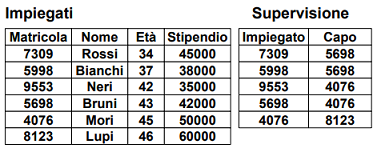
\includegraphics{img/60.PNG}
\end{center}  
\begin{verbatim}
	readelf -Wl main
\end{verbatim}
Interpreto ogni riga nel seguente modo: carica a partire dall'offset \emph{Offset} del file all'indirizzo \emph{VirtAddr}, carica \emph{FileSiz} byte, azzera ulteriori byte arrivando fino \emph{memSiz} byte (se $\text{\emph{FileSiz}} = \text{\emph{memSiz}}$ non si azzera nulla di più rispetto alla dimensione del file), successivamente faccio quanto indicato dai \emph{Flg}.

\section{Librerie statiche}
In UNIX una libreria consiste in un archivio di file oggetto.
\paragraph{Riflessione} Prendiamo tre files assembler: \emph{foo.s}, \emph{bar.s}, \emph{main2.s}. Il contenuto del secondo file non viene utilizzato negli altri due. Per prima cosa creiamo i files oggetto
\begin{verbatim}
	g++ -c foo.s bar.s main2.s
\end{verbatim}
successivamente colleghiamo col linker
\begin{verbatim}
	ld -o main main2.o foo.o bar.o
\end{verbatim}
Tutti i files vengono uniti, indipendentemente dall'utilizzo delle funzioni. Cioè, posso unire a un set di files oggetto un ulteriore file oggetto con funzioni che non utilizziamo negli altri files.
\subsection{Come si crea una libreria?} Col seguente comando
\begin{verbatim}
	ar cr mialib.a foo.o bar.o
\end{verbatim}
andiamo a creare un archivio, un unico file che contiene al suo interno altri files e presenta un'intestazione che permette di capire cosa è effettivamente presente nell'archivio. Il file creato (in GNU) è già pronto per essere usato.
\clearpage
\subsection{Comandi utilizzati fino ad ora e librerie}
I files archivio \emph{a} sono ben noti dai programmi che abbiamo già visto. Vediamo alcuni esempi.
\begin{multicols}{2}
	\paragraph{Lettura dell'intestazione ELF}
	\begin{verbatim}
		readelf -h mialib.a
	\end{verbatim}
	\begin{center}
		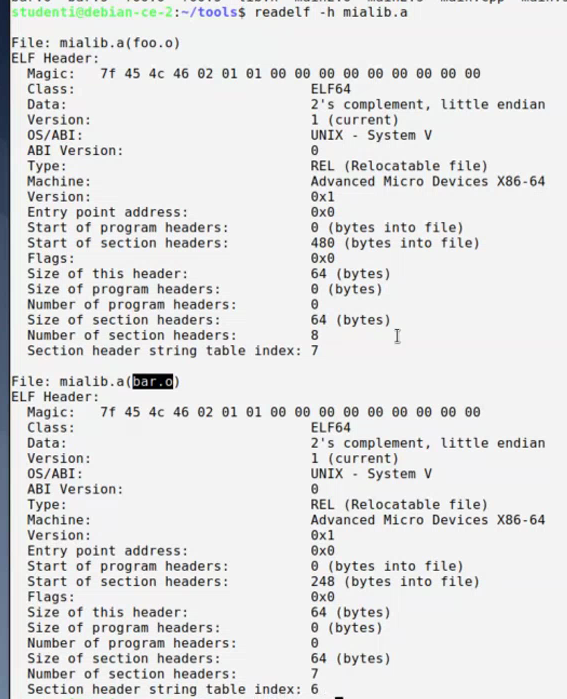
\includegraphics[scale=0.70]{img/61.png}
	\end{center}
	\columnbreak
	\paragraph{objdump}
	\begin{verbatim}
		objdump -d mialib.a
	\end{verbatim}
	\begin{center}
		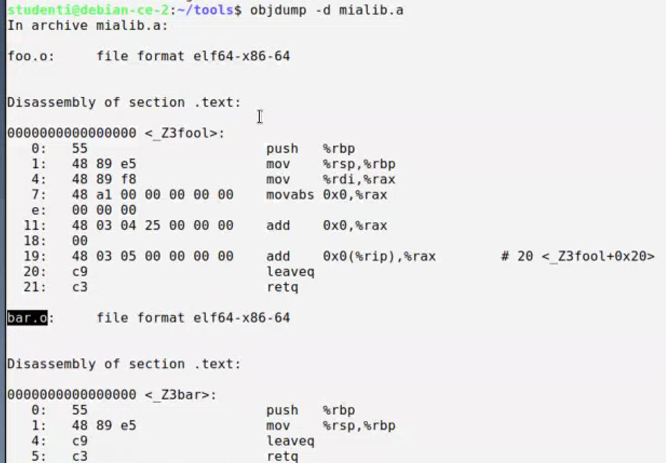
\includegraphics[scale=0.65]{img/62.png}
	\end{center}
\end{multicols}
\paragraph{nm} Possiamo fare di più
\begin{verbatim}
	nm -s mialib.a
\end{verbatim}
\begin{center}
	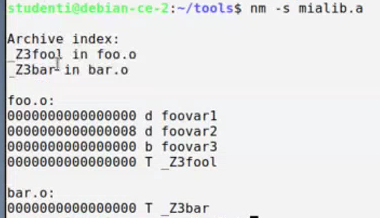
\includegraphics{img/63.png}
\end{center}
Con l'opzione $-\text{s}$ possiamo vede l'indice che è stato creato nell'archivio: possiamo distinguere simboli globali e simboli locali, e vedere in che file sono stati definiti i simboli globali.

\paragraph{ld} A questo punto posso collegare la mia libreria con il file \emph{main.o}
\begin{verbatim}
	ld -o main main2.o mialib.a
\end{verbatim}
Ricerca nella libreria soltanto i simboli non definiti: per ogni simbolo non definito si porta dentro il corrispondente file oggetto. Il resto è uguale a prima. Se noi proviamo a usare \emph{objdump} vedremo che sono state prese solo le cose necessarie (\emph{bar}, l'intruso, non è più presente). Attenzione: conseguenza di quanto detto è che se noi invertiamo nel comando l'ordine dei file assemblati avremo errore. Convenzione vuole che le librerie vadano \underline{SEMPRE} in fondo, in modo tale da considerare solo le cose che effettivamente ci servono (possiamo sapere cosa ci serve solo se processiamo gli altri files oggetto prima delle librerie).
\paragraph{Directories per le librerie} Il linker è in grado di andare a cercare automaticamente le librerie in una serie di cartelle, in un certo senso come il preprocessore. Vediamo alcuni esempi
\begin{verbatim}
	ls /usr/include/
	ls /usr/lib/
	ls /usr/local/lib/
\end{verbatim}
La convenzione UNIX richiede che il nome cominci per \emph{lib}. Inoltre, per copiare in quelle cartelle dobbiamo diventare amministratori. Copiamo utilizzando un comando leggermente diverso (viene richiesta la password, svolgiamo l'operazione come amministratore)
\begin{verbatim}
	sudo cp mialib.a /usr/local/lib/libmia.a
\end{verbatim}
nel comando per collegare richiameremo la libreria così
\begin{verbatim}
	ld -o main main2.o -lmia
\end{verbatim}
Attenzione a \emph{lib} abbreviato con \emph{l}. Per quanto riguarda \emph{g++}, che tra tante cose utilizza \emph{ld}, dobbiamo scrivere il seguente comando
\begin{verbatim}
	g++ -no-pie -nostdlib -o main main2.o -lmia
\end{verbatim}
